\subsubsection{Superstar}

\zadatak
Doka{\zv}i da za $x>0$ va{\zv}i najpoznatija logaritamska nejednakost
$$
1-\frac1x \le \ln x \le x - 1.
$$

\resenje
Pogledajmo prvo desnu stranu nejednakosti. Ako defini{\sv}emo funkciju
$$
y=\ln x - (x - 1) = \ln x - x + 1,
$$
potrebno je da doka{\zv}emo da je $y\le0$ za svako $x$.
Prvi izvod funkcije je
$$
y' = \frac1x - 1
$$
koji ima jedinstvenu nulu za $x=1$. Kako je drugi izvod
$$
y''=-\frac1{x^2}<0,\quad \forall x>0,
$$
to zna{\cv}i da funkcija $y$ nema {\sl prevojnih ta{\cv}aka\/} i da je u ta{\cv}ki $(1,0)$ {\sl maksimum\/} funkcije  $y$,
odakle je $y\le0$, odnosno,
$$
\ram{\ln x \le x - 1}.
$$
Ako u ovu nejednakost umesto $x$ stavimo $1/x$, mo{\zv}emo pisati
\begin{align*}
    \ln(1/x) &\le \frac1x -1 \\
    -\ln x &\le \frac1x -1, 
\end{align*}
gde, kada izrazi zamene strane, dobijamo
$$
    \ram{1-\frac1x \le \ln x},
$$
{\sv}to predstav{\lj}a levu stranu nejednakosti.\hfill\QED

$$
\slika{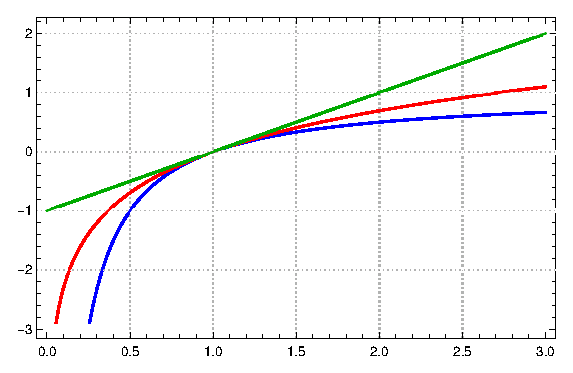
\includegraphics[width=80mm]{eps/royal.eps}}{$
{\color{blue}y=1-1/x};\
{\color{red}y=\ln x};\
{\color{Green}y=x-1}
.$}
$$

\dodatak Za $x=1$, sve tri strane se {\sl dodiruju\/} u $y=0$, {\sv}to zna{\cv}i da
u toj ta{\cv}ki sve tri imaju istu {\sl tangentu}, odnosno, isti prvi izvod $y'=1$, 
{\sv}to se lako dokazuje,
ina{\cv}e
bi se sekle i nejednakost ne bi va{\zv}ila.

